\chapter{Практика}
\label{ch:chap2}

\section*{\textbf{Задание 1: выполнить ППФ над прямоугольным сигналом (на бумаге)}}

\begin{figure}[H]
    \centering
    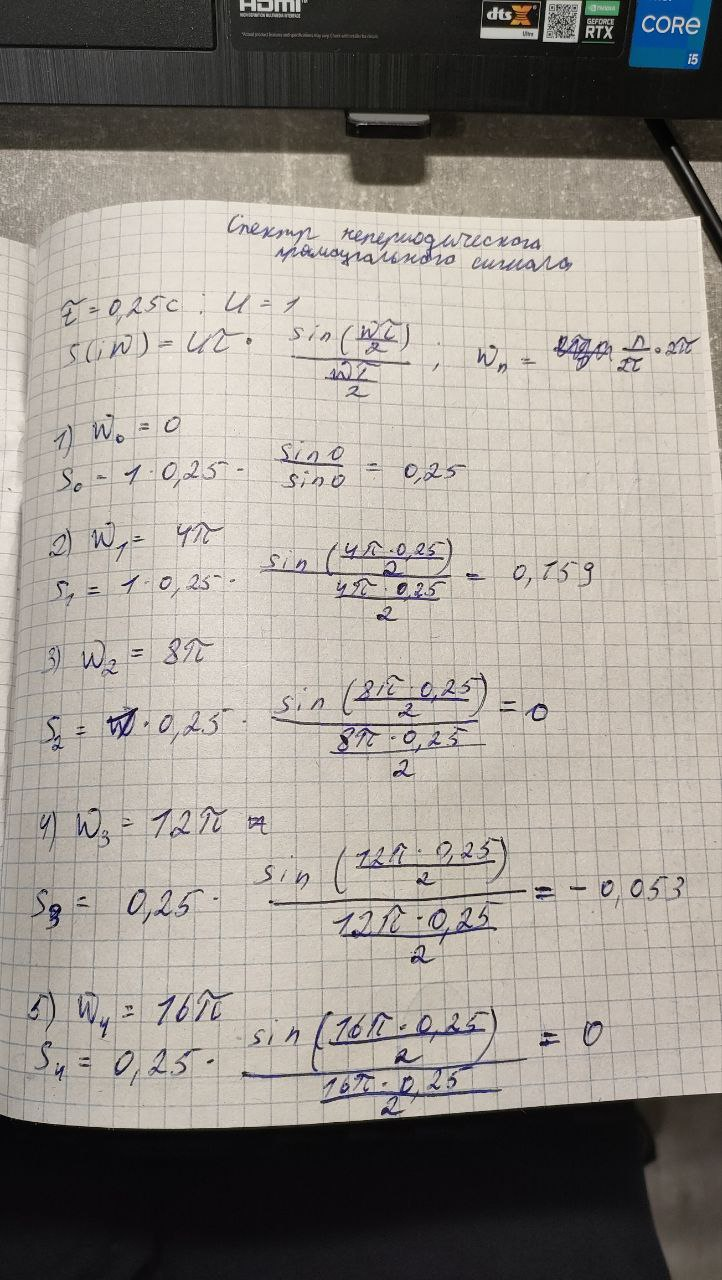
\includegraphics[width=1.0\textwidth]{dz.jpg}
    \caption{Вычисления}
\end{figure}

\begin{figure}[H]
    \centering
    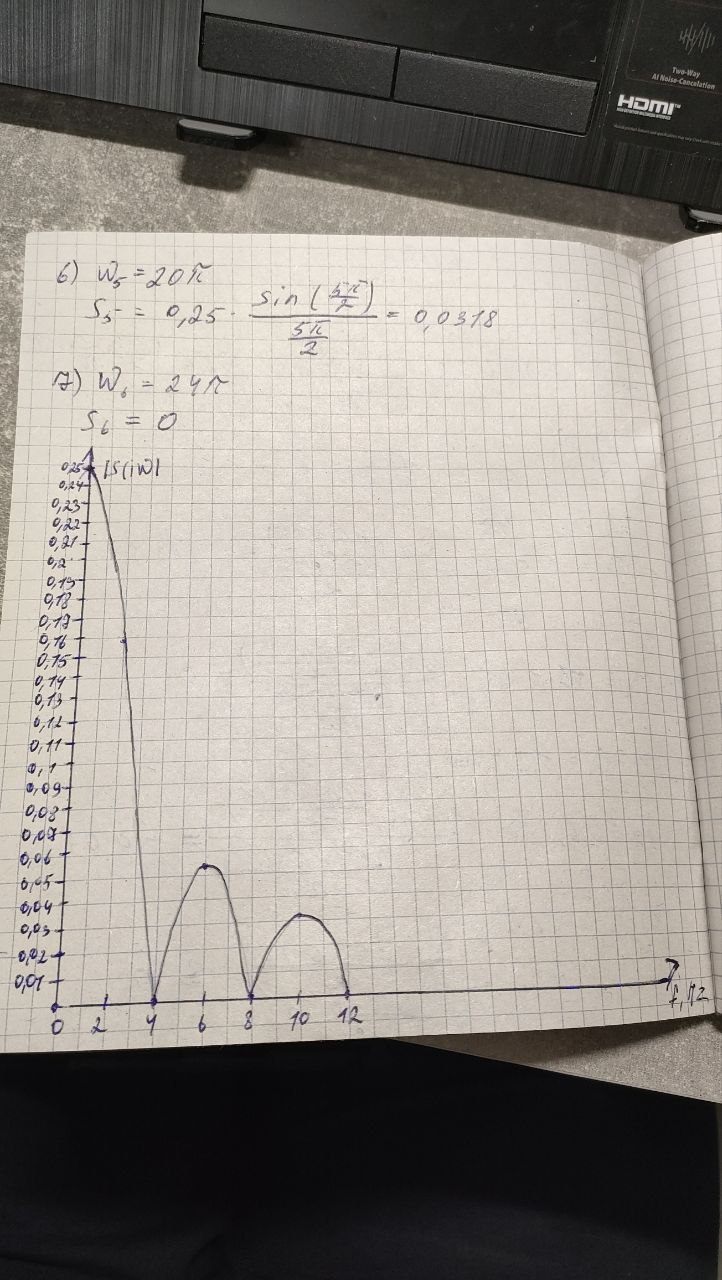
\includegraphics[width=1.0\textwidth]{dz2.jpg}
    \caption{Вычисления}
\end{figure}

\section*{\textbf{Задание 2: выполнить ППФ над прямоугольным сигналом}}

Выполним ППФ по формуле $S(i\omega) = \int_{-\infty}^{\infty}S(t)e^{i\omega \tau} d\tau$. Пределы интеграла изменятся на 
[$-\frac{\tau}{2};\frac{\tau}{2}$]. Интегрировать будем численно: суммируем подынтегральную функцию 
$S(t)e^{i\omega \tau}$ в каждый момент времени t, а потом умножаем на $dt$. Для графика ниже $\tau = 0.25$

\begin{figure}[H]
    \centering
    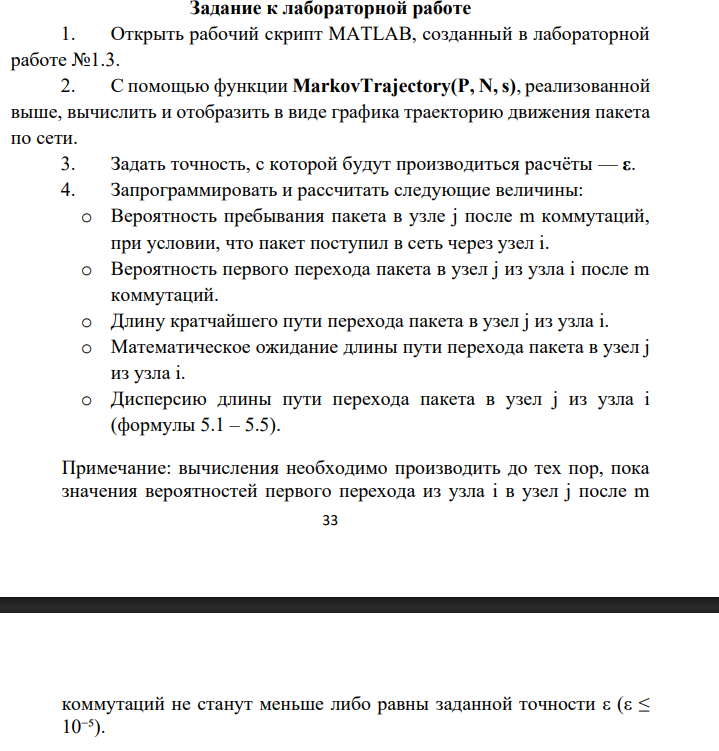
\includegraphics[width=1.0\textwidth]{task1.png}
    \caption{Моудль и аргумент спектральной функции прямоугольного сигнала}
\end{figure}

График такой же, как и на прошлом шаге, когда вычисления происходили вручную. График имеет вид функции $\frac{sin(x)}{x}$.

\section*{\textbf{Задание 3: проверка свойства ППФ прямоугольного сигнала с измением длительности сигнала}}

В этом задании увеличим, а потом уменьшим длительность сигнала $\tau$ и посмотрим на результат.

\begin{figure}[H]
    \centering
    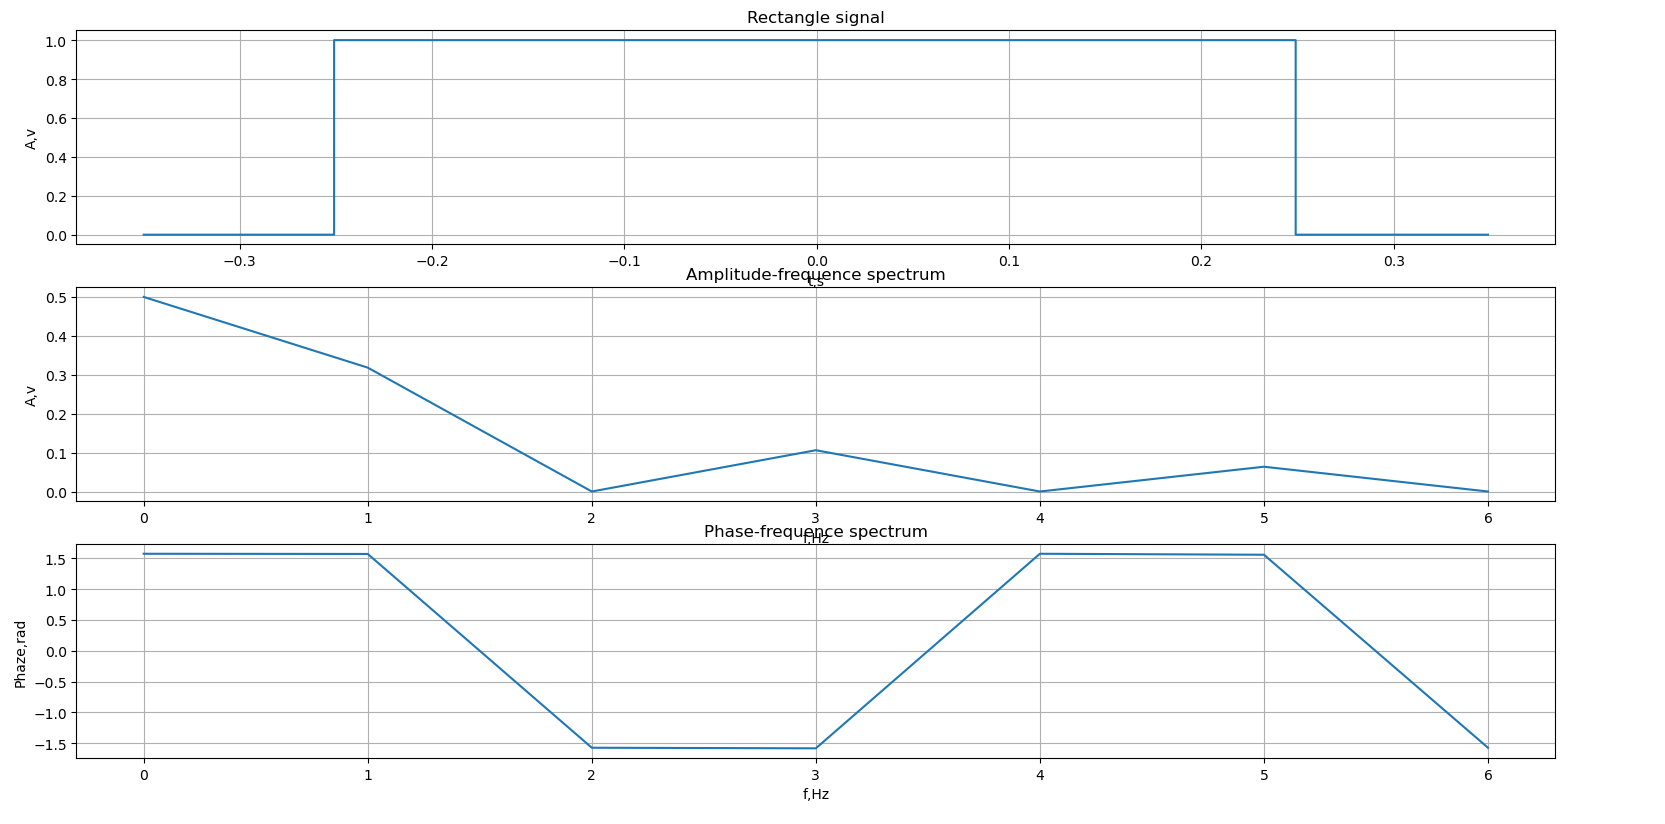
\includegraphics[width=1.0\textwidth]{tau05.png}
    \caption{$\tau = 0.5$}
\end{figure}

\begin{figure}[H]
    \centering
    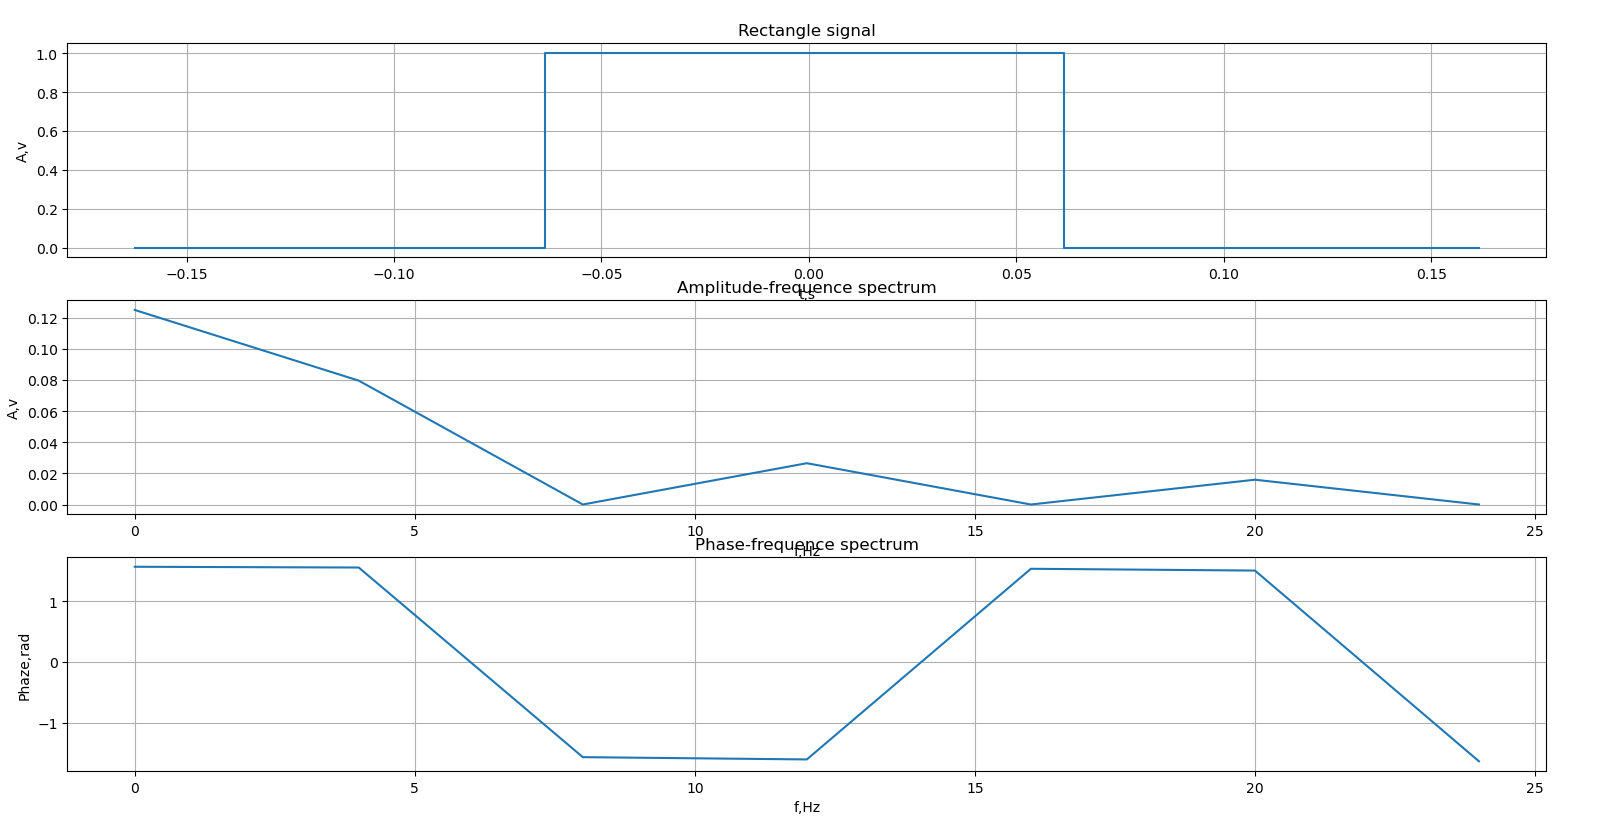
\includegraphics[width=1.0\textwidth]{tau0125.png}
    \caption{$\tau = 0.125$}
\end{figure}

Можем заметить, что при уменьшении $\tau$ вдвое, спектр становится шире в два раза. Если увеличиваем длительность вдвое, то спектр
сужается вдвое. Это следует из формулы $\triangle \omega = \frac{n}{2\tau}$. При увеличении длительности сигнала знаменатель дроби
растет, поэтому шаг становится меньше и при одинаковом интервале частот график сузится. При уменьшении $\tau$ шаг растет и график
растягивается. Точки, в которых спектральная функция принимает значение 0 (на частотах кратных $\frac{1}{\tau}$) тоже смещаются.

\section*{\textbf{Задание 4: проверка свойства ППФ задержанного прямоугольного сигнала}}

Для проверки свойства введем переменную, которая будет отвечать за двиг сигнала во времени. В моем случае сдвиг будет на 0.1 секунды.

\begin{figure}[H]
    \centering
    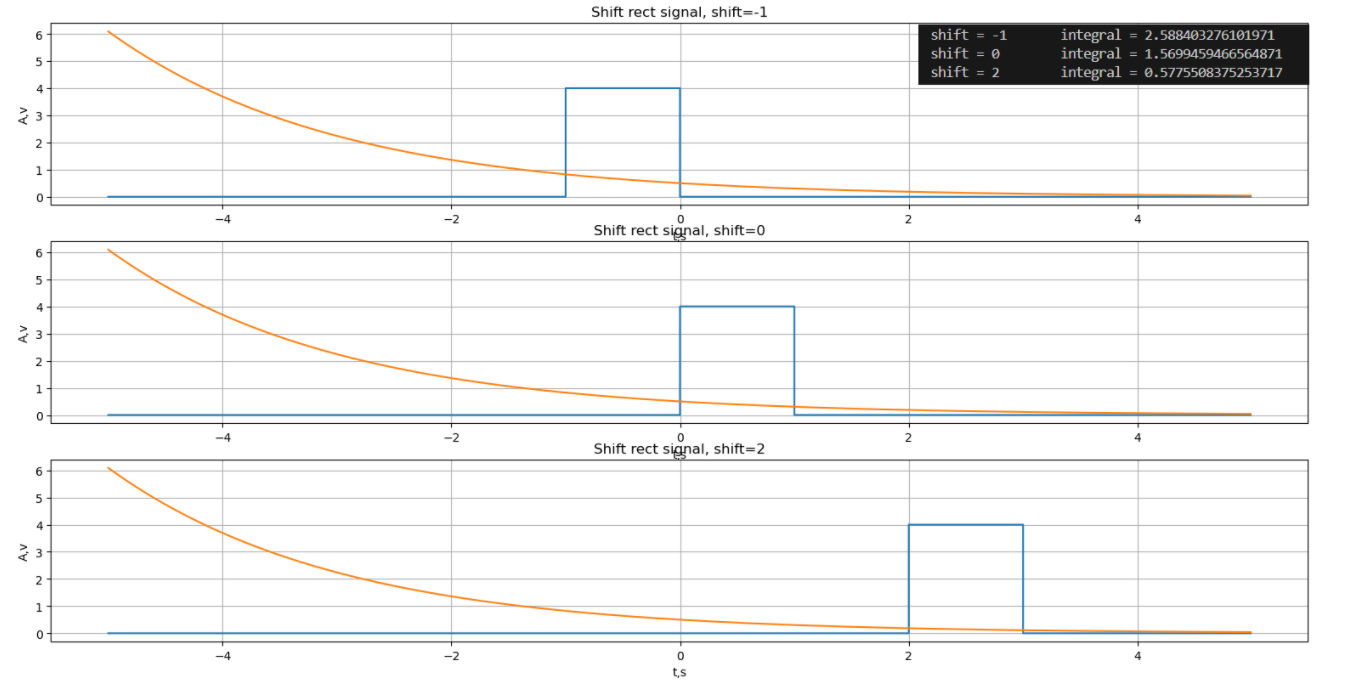
\includegraphics[width=1.0\textwidth]{shift.png}
    \caption{Прямоугольный сигнал, сдвинутый во времени}
\end{figure}

Видим, что амплитудный спектр никак не изменился, а изменился только фазовый спектр. Эти изменения вносит множитель $e^{-i\omega t_0}$,
где $t_0$ - время сдвига. Теоретически, если я разделю получившуюся спектральную функцию на $e^{-i\omega t_0}$, то спектр должен вернуться
к исходному виду (первый скриншот, где $\tau = 0.25$).

\begin{figure}[H]
    \centering
    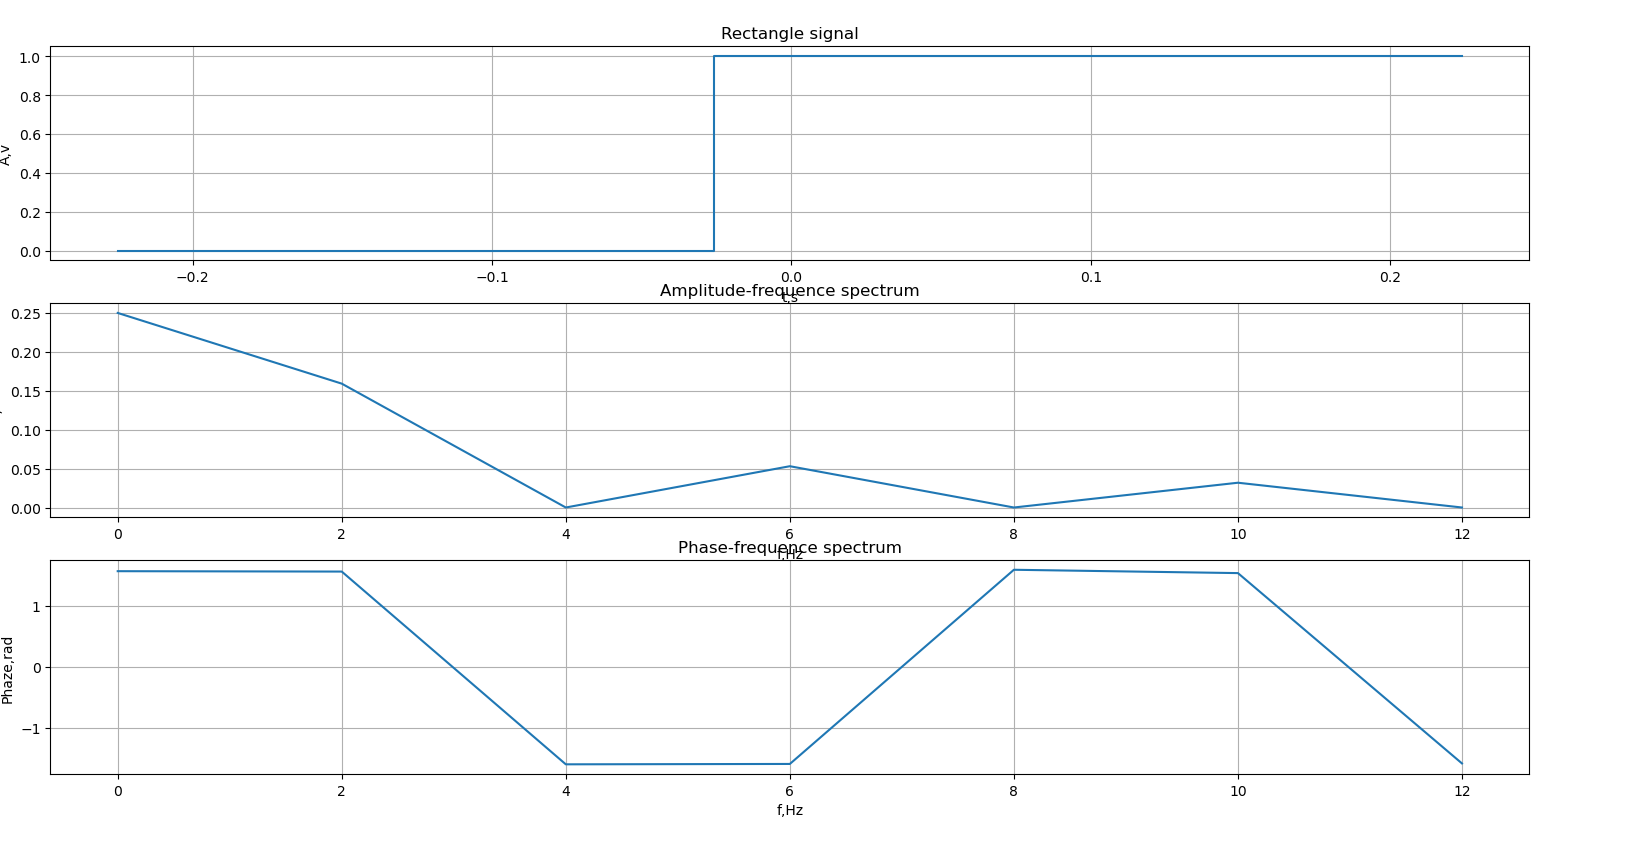
\includegraphics[width=1.0\textwidth]{fix_shift.png}
    \caption{Демонстрация свойства задержанного сигнала}
\end{figure}

Можем видеть, что спектр вернулся в исходное состояние.

\section*{\textbf{Задание 5: проверка свойства ППФ прямоугольного сигнала (свойство модуляции, смещения спектра)}}

Для проверки свойства умножим исходный сигнал на $e^{i\omega_0t}$, таким образом спектр сигнала сдвинется на $\omega_0$ и это можно
будет увидеть на графике.

\begin{figure}[H]
    \centering
    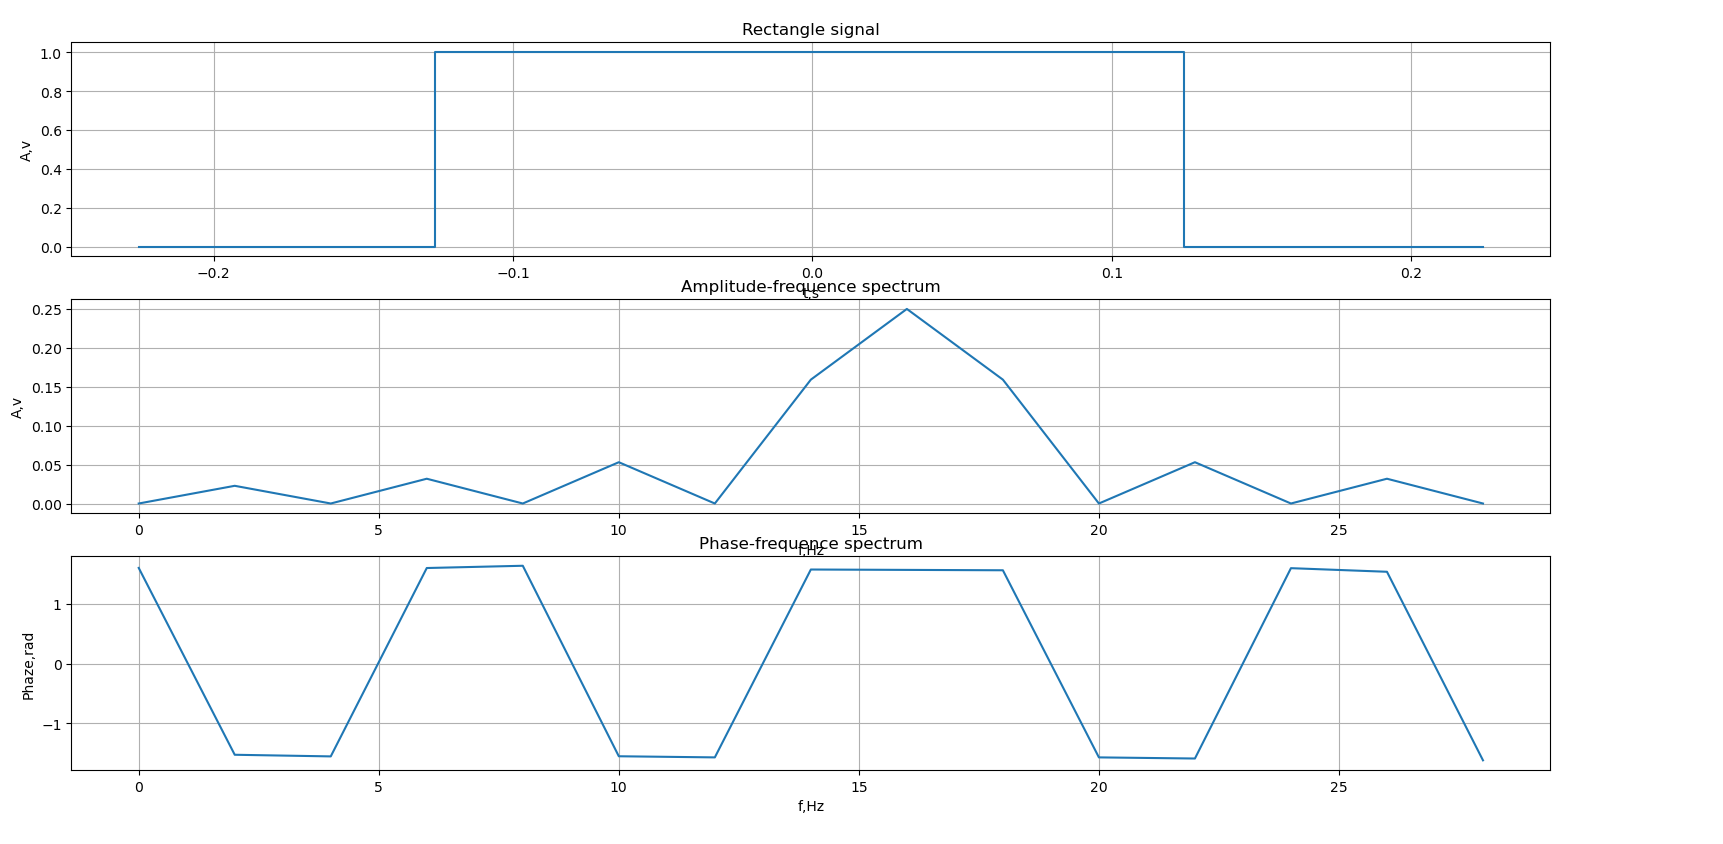
\includegraphics[width=1.0\textwidth]{shift_signal.png}
    \caption{Демонстрация свойства модуляции сигнала}
\end{figure}

Можем видеть, что сигнал действительно сдвинулся вправо на 16 Hz, именно 16 Hz я и задавал для сдвига. Также можно заметить, что
фазовый спектр тоже изменился.

\section*{\textbf{Приложение}}

Листинг кода:
\begin{lstlisting}
import matplotlib.pyplot as plt
import numpy as np

# define rect signal param

# set time shift
t0 = 0

tau = 0.25
dt = 0.001
ofset = 0.1

# define rect signal

start = -tau/2 - ofset
end = tau/2 + ofset

timeline = np.arange(start,end,dt)

signal = [1 if i <= tau/2 + t0 and i >= -tau/2 + t0  else 0  for i in timeline]


plt.subplot(3, 1, 1)
plt.step(timeline, signal)
plt.xlabel("t,s")
plt.ylabel("A,v")
plt.title("Rectangle signal")
plt.grid()

# FT on [0, 3/tau]
N = 15
ft_result = []
f_ax = []

w_0 = 0

# uncomment if you want shift signal
#w_0 = 16 * 2 * np.pi

for i in range(0, N):
    
    w = i*1/(2 *tau) * 2 * np.pi
    
    f_ax.append(w / (2 * np.pi))
    
    e = np.exp(-1j * w * timeline)
    
    e_shift = np.exp(1j * w_0 * timeline)

    # S(t) * e^(-iwt)
    integral_func = signal * e * e_shift
    
    # numerical integration
    
    ft_result.append(np.sum(integral_func) * dt) 
    
    
plt.subplot(3, 1, 2)
plt.plot(f_ax, list(map(abs, ft_result)))
plt.xlabel("f,Hz")
plt.ylabel("A,v")
plt.title("Amplitude-frequence spectrum")
plt.grid()

plt.subplot(3, 1, 3)
plt.plot(f_ax, list(map(np.arctan2, [x.real for x in ft_result], [x.imag for x in ft_result])))
plt.xlabel("f,Hz")
plt.ylabel("Phaze,rad")
plt.title("Phase-frequence spectrum")
plt.grid()
plt.show()




\end{lstlisting}

\endinput